\subsection{Ziel}

Automatisches Schlussfolgern spielt eine zentrale Rolle für BLen. Insbesondere ist die Ausdruckstärke von BLen stark darauf zugeschnitten.

Dabei ist aber wichtig, dass die relevanten Schlussfolgerungsprobleme entscheidbar sind, sie ein möglichst geringe Komplexität haben und/oder Algorithmen existieren, die sich in der Praxis performant verhalten.

Von uns wird hauptsächlich das Problem der Erfüllbarkeit betrachtet.

In der Praxis haben sich hauptsächlich Tableau-Algorithmen und Resolutionsverfahren als effizient herausgestellt.

\subsection{ALC ohne TBoxen}\label{alc-ohne-tboxen}

\subsubsection{Negationsnormalform}\label{negationsnormalform}

\begin{definition}{Negationsnormalform}

Konzept ist in \emph{Negationsnormalform} (NNF) gdw. Negation nur auf
Konzeptnamen angewendet wird.
\end{definition}

\begin{lemma}
Jedes Konzept kann in Linearzeit in ein äquivalentes Konzept in NNF
umgewandelt werden.
\end{lemma}

\textbf{T4.1}

Beweisskizze. Wende Gesetze der doppelten Negation, de Morgan und
Dualität von $\exists$, $\forall$ an.

\subsubsection{I-Baum}\label{i-baum}

\begin{definition}{I-Baum}

\emph{I-Baum} für $C_{0}$ (in NNF) ist knoten- und kantenbeschrifteter
Baum $\left( V,E,L \right)$ mit

\begin{itemize}
\item
  $V$ Knotenmenge
\item
  $E$ ist Menge beschrifteter Kanten $\left( v,r,v^{'} \right)$ mit
  $v$,$\ v^{'} \in V$, $r$ Rollenname
\item
  $L$: $V \rightarrow 2^{sub(C_{0})}$
\end{itemize}
\end{definition}

\textbf{T4.2}

Bsp. $$C_0 = A \sqcap \forall r.(\neg A \sqcap \exists r.B)$$
$$sub(C_0) = \{A, \neg A, B, \exists r.B, \neg A \sqcap \exists r.B, \forall r.(\neg A \sqcap \exists r.B)\}$$

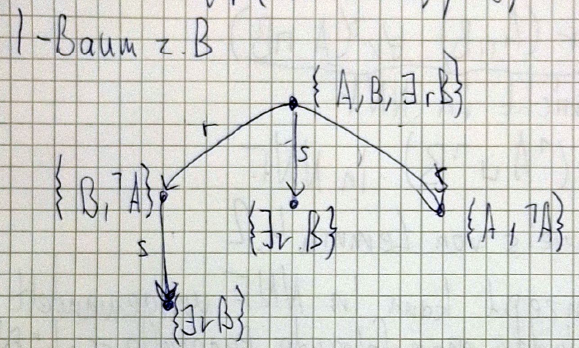
\includegraphics[width=3.71910in,height=1.83200in]{media/42ibaum.png}

\subsubsection{Tableau-Algorithmus}\label{tableau-algorithmus}

Berechnet Folge $$M_{0},M_{1},\ldots$$ von Mengen von I-Bäumen:

$$M_{0} = \left\{ B_{\text{ini}} \right\}\ mit\ B_{\text{ini}}\ \emph{initialer I-Baum}\ fuer\ C_{0}:$$

\begin{itemize}
\item
  $V := \left\{ v_{\text{ini}} \right\}$
\item
  $E := \emptyset$
\item
  $L := \left( v_{\text{ini}} \right) \left\{ C_{0} \right\}$
\end{itemize}

$M_{i + 1}$ entsteht aus $M_{\MI}$ durch Anwendung der Tableau-Regeln
auf irgendeinen I-Baum in $M_{\MI}$ und anschließendes Austauschen des
verwendeten Baumes durch den neu erzeugten (Sei $\left( V,E,L \right)$
I-Baum):

\begin{itemize}
\item
  $\sqcap$-Regel

  \begin{itemize}
  \item
    Wähle $v \in V$ und $C \sqcap D \in L\left( v \right)$ so dass
    \emph{nicht} $\left\{ C,D \right\}\  \subseteq L\left( v \right)$
  \item
    erweitere $L(v)$ um $C$ und $D$
  \end{itemize}
\item
  $\sqcup$-Regel

  \begin{itemize}
  \item
    Wähle $v \in V$ und $C \sqcup D \in L\left( v \right)$ so dass
    $\left\{ C,D \right\}\  \cap L\left( v \right) = \varnothing$
  \item
    erweitere $L(v)$ um $C$ oder $D$ (ergibt zwei I-Bäume)
  \end{itemize}
\item
  $\exists$-Regel

  \begin{itemize}
  \item
    Wähle $v \in V$ und $\exists r.C \in L\left( v \right)$ so dass
    es kein $v^{'} \in V$ gibt mit $\left( v,r,v^{'} \right) \in E$
    und $C\  \in L\left( v' \right)$
  \item
    erweitere V um neuen Konten $v^{'}$ und $E$ um
    $\left( v,r,v^{'} \right)$; setze
    $L\left( v^{'} \right) = \left\{ C \right\}$
  \end{itemize}
\item
  $\forall$-Regel

  \begin{itemize}
  \item
    Wähle $v,v^{'} \in V$ und $\forall r.C \in L\left( v \right)$ so
    dass $\left( v,r,v^{'} \right) \in E$ und
    $C\  \notin L\left( v \right)$
  \item
    erweitere $L(v')$ um $C$
  \end{itemize}
\end{itemize}

Stoppe, wenn alle Regeln erschöpfend angewandt wurden. Gib „erfüllbar``
zurück, falls es einen I-Baum ohne offensichtlichen Widerspruch
($\left\{ A,\neg A \right\} \subseteq L\left( v \right)$) gibt;
„unerfüllbar`` sonst.

\textbf{T4.3}

Beispiel:

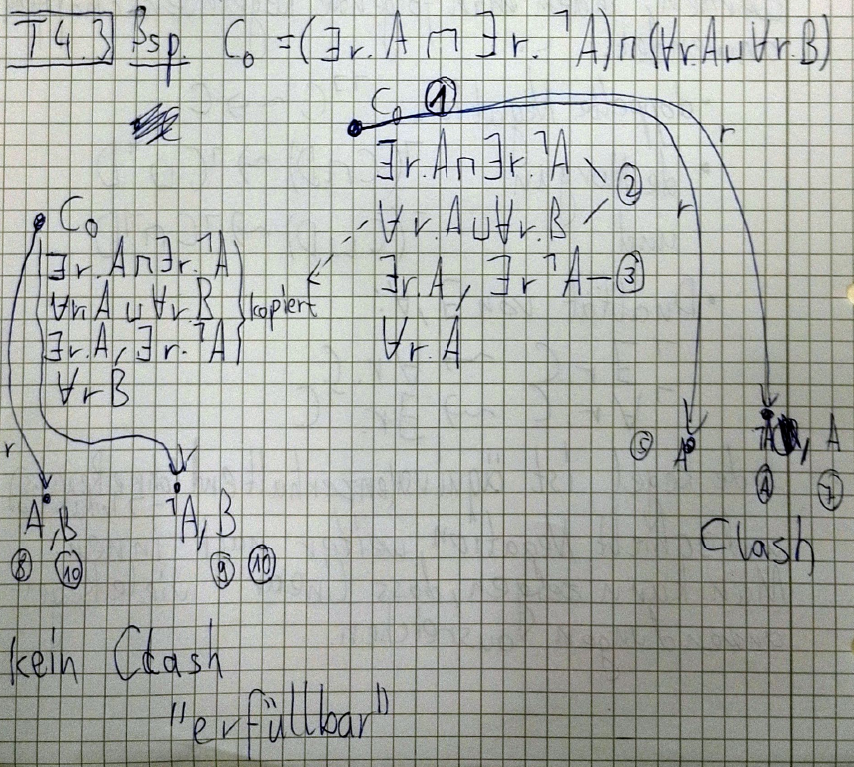
\includegraphics[width=5.71910in,height=3.83200in]{media/43taleau.png}

\subsubsection{Definition Rollentiefe}\label{definition-rollentiefe}

Rollentiefe $\text{rd}\left( C \right)$ von Konzepten
$C \in sub\left( C_{0} \right)$ ist induktiv definiert:

\begin{itemize}
\item
  $\text{rd}\left( A \right) = rd\left( \neg A \right) = 0$
\item
  $\text{rd}\left( C \sqcap D \right) = rd\left( C \sqcup D \right) = \max\left( \text{rd}\left( C \right),rd\left( D \right) \right)$
\item
  $\text{rd}\left( \exists r.C \right) = rd\left( \forall r.C \right) = 1 + rd\left( C \right)$
\end{itemize}

\begin{lemma}
Für alle $C \in sub\left( C_{0} \right)$ gilt
$\text{rd}\left( C \right) \leq \left| C \right|$.
\end{lemma}

\subsubsection{Multimengen}\label{multimengen}

Multimengen sind Mengen, in denen Elemente mehrfach vorkommen dürfen, z.B.:
$$\{1,1,2,3,4,4,5,6,6,6\}$$

Formal: Multimengen über die Menge $S$ ist Abbildung $$M:S\mathbb{\rightarrow N}$$, welche jedes Element auf die Anzahl seines Vorkommens abbildet.

Die meisten Begriffe übertragen sich von Mengen auf Multimengen:

\begin{itemize}
	\item Leere Menge $\emptyset: s \mapsto 0$ für alle $s \in S$
	\item Vereinigung $(M_1 \cup M_2)(s) := M_1(s) + M_2(s)$ 
	\item Element: $s \in M\ gdw.\ M(s)>0$
	\item Differenz: $(M_1 \setminus M_2)(s) = X(m,n) = \left\{\begin{array}{lr}
        M_1(s) - M_2(s) &, wenn M_1(s) \geq M_2(s) \\
        0 & sonst
        \end{array}\right\}$
\end{itemize}

$MM(S)$ ist die Menge aller Multimengen über der Menge S.

Gegeben strikte partielle Ordnung $\left( S, < \right)$, ist die
\emph{Multimengenerweiterung} $\left( \text{MM}\left( S \right), <_{\text{mul}} \right)$ definiert als: 

$M_{2} <_{\text{mul}}M_{1}$ gdw. $\exists X,Y \in MM(S)$, so dass

\begin{itemize}
\item
  $\varnothing \neq X \subseteq M_{1}$
\item
  $M_{2} = \left( M_{1} \smallsetminus X \right) \cup Y$
\item
  $\forall y \in Y\exists x \in X : x > y$
\end{itemize}

Also erhält man $M_2$ aus $M_1$, indem man einige Elemente entfernt und durch endlich viele \emph{kleinere} ersetzt.

Beispiel:

$\left\{ 3,1 \right\} >_{\text{mul}}\{ 2,2,2\} >_{\text{mul}}\{ 2,2\} >_{\text{mul}}\{ 2,1,1,1\}$

Es ist leicht zu zeigen das diese Ordnung eine strikte partielle Ordnung ist.  Zudem ist sie wohlfundiert, wenn $(S,<)$ wohldefiniert ist: Es gibt keine unendlich $<$ absteigenden Ketten.

\setcounter{definition}{5}
\begin{theorem}

Wenn $\left( S, < \right)$ wohlfundiert (hat keine unendlichen
absteigenden Ketten) ist, dann ist auch $\left( \text{MM}\left( S \right), <_{\text{mul}} \right)$
wohlfundiert.
\end{theorem}

\setcounter{definition}{4}

\subsubsection{Terminierung}

\begin{proposition}

Der Tableau-Algorithmus stoppt nach endlicher Zeit.
\end{proposition}
\setcounter{definition}{6}

Beweis in 4 Schritten:

\begin{enumerate}
\def\labelenumi{\arabic{enumi}.}
\item
  Es werden nur I-Bäume mit einem Verzweigungsgrad
  $\leq \left| C_{0} \right|$ generiert.

\begin{quote}
\textbf{T4.5a}

Beweisskizze. Nur die $\exists$-Regel generiert Nachfolger, aber
höchstens einen für jedes Konzept $\exists r.C \in sub(C_{0})$. Nach
\protect\hyperlink{lemma-3.13}{Lemma 3.13} enthält
$\text{sub}\left( C_{o} \right)$ höchstens $\left| C_{0} \right|$
viele Konzepte.
\end{quote}

\def\labelenumi{\arabic{enumi}.}
\item
  Es werden nur I-Bäume mit einer Tiefe $\leq \left| C_{0} \right|$
  generiert.

\begin{quote}
\textbf{T4.5b}
\begin{proof}

Induktion über die Anzahl der Regelanwendungen. Zu zeigen: Wenn $v$
Knoten mit Tiefe $\MI$ ist, dann gilt
$\text{rd}\left( C \right) \leq rd\left( C_{0} \right) - i$ für alle
$C \in L\left( v \right)$.

\textbf{I.A.} Es gibt nur Knoten $v_{\text{ini}}$ mit
$L\left( v_{\text{ini}} \right) = \left\{ C_{0} \right\}$. I.V. gilt,
da $i = 0$.

\textbf{I.S.} Fallunterscheidung nach angewandter Regel (exemplarisch
$\sqcap$, $\exists$):

\begin{enumerate}
\def\labelenumi{\alph{enumi}.}
\item
  $\sqcap$-Regel

$C \sqcap D \in L(v)$ und $L(v)$ wird durch $C$, $D$ erweitert.
Nach I.V. gilt:
$\text{rd}\left( C \sqcap D \right) \leq rd\left( C_{0} \right) - i$,
also auch $\text{rd}\left( C \right) \leq rd\left( C_{0} \right) - i$,
weil $\text{rd}\left( C \right) \leq rd\left( C \sqcap D \right)$.
Analog für $D$.

\def\labelenumi{\alph{enumi}.}
\item
  $\exists$-Regel

Dann $\exists r.C \in L\left( v \right)$ und es wird neues $v^{'}$
auf Tiefe $i + 1$ generiert mit
$L\left( v^{'} \right) = \left\{ C \right\}$. Es gilt
$\text{rd}\left( C \right) = rd\left( \exists r.C \right) - 1 \leq rd\left( C_{0} \right) - i - 1 = rd\left( C_{0} \right) - (i + 1)$
 \end{enumerate}
\end{proof}
\end{quote}

\item
  Sei $M_{0},M_{1},\ldots$ die erzeugte Folge und $B \in M_{\MI}$ für
  ein $i \geq 0$. Dann ist $B$ durch die Anwendung von maximal
  $\left| C_{0} \right|^{\left| C_{0} \right|} \cdot \left| C_{0} \right| \leq 2^{2\left| C_{0} \right|^{2}} = n$ Regeln entstanden (Knoten im Baum mal Größe Knotenbeschriftung).

\end{enumerate}

Nun kann die Terminierung mittel Behauptung 3 beweisen:

\textbf{T4.5d}

\begin{proof}
Wir ordnen jedem $M_i$ eine Multimenge $MM_i$ zu. Für jedes $B \in M_i$ enthält $MM_i$ die Zahl der ``n$-$Anzahl der Regelanwendungen, mittels derer $B$ generiert wurde.''

Weil $<$ auf $\mathcal{N}$ wohldefiniert ist, ist $<_{mul}$ auf $MM(\{0,\ldots,n\})$ wohldefiniert.

Offenbar gilt $MM_{i+1} <_{mul} MM_i$ für alle $i \geq 0$ *. Also werden nur endlich oft Regeln angewendet.
\end{proof}

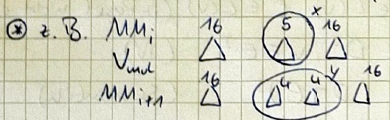
\includegraphics[width=3.71910in,height=1.83200in]{media/45mm.png}

\subsubsection{Korrektheit und Vollständigkeit}

\begin{proposition}

Wenn der Tableau-Algorithmus „erfüllbar`` zurückgibt, so ist $C_{0}$
erfüllbar.
\end{proposition}

\textbf{T4.6}

\begin{proof}

Beweis per Induktion über die Struktur von $C$.
„erfüllbar``-Ausgabe bedeutet widerspruchsfreier, vollständiger I-Baum
$B = \left( V,E,L \right)$ gefunden. Konstruiere Interpretation $\MI$:

\begin{itemize}
\item
  $\Delta^{\MI} = V$
\item
  $r^{\MI} = \left\{ \left( v,v^{'} \right) \middle| \left( v,r,v^{'} \right) \in E \right\}$
  für alle Rollennamen $r$
\item
  $A^{\MI} = \left\{ v \middle| A \in L\left( v \right) \right\}$ für
  alle Konzeptnamen $A$
\end{itemize}

Behauptung: Für alle Konzepte $C$ und $v \in V$ gilt

\begin{center}$C \in L\left( v \right)$ impliziert $v \in C^{\MI}$\end{center}

Da $C_{0} \in L\left( v_{\text{ini}} \right)$ in $B_{\text{ini}}$ gilt
auch $C_{0} \in L\left( v_{\text{ini}} \right)$ in $B$. Also
$v_{\text{ini}} \in C_{0}^{\MI}$ nach Behauptung, weswegen dann
$C_{0}$ erfüllbar.

\textbf{I.A.} $C = A$ (Konzeptname) Gilt nach Definition von
$\MI$.

\textbf{I.S.}

\begin{itemize}
\item
  $C = \neg A$

\begin{quote}
$A$ Konzeptname. Da $B$ keinen offensichtlichen Widerspruch hat,
folgt das $A \notin L(v)$. Nach Definition von $\MI$ gilt
$v \notin A^{\MI}$. Also $v \in \left( \neg A \right)^{\MI}$.
\end{quote}

\item
  $C = D \sqcap E$

\begin{quote}
$C \in L\left( v \right)$ 

$\Rightarrow$ ($\sqcap$-Regel nicht anwendbar) $D \in L\left( v \right),\ E \in L\left( v \right)$ 

$\Rightarrow$ (I.V.) $v \in D^{\MI},\ v \in E^{\MI}$ 

$\Rightarrow$ (Semantik) $v \in \left( D \sqcap E \right)^{\MI}$
\end{quote}

\item $C = D \sqcup E$

\begin{quote}
analog.
\end{quote}

\item $C = \exists r.D$

\begin{quote}
Da die $\exists$-Regel nicht anwendbar ist, gibt es $v'\in V$ mit $(v,r,v') \in E$ und $D \in L(v')$

Nach I.V.: $v' \in D^{\MI}$; nach Konstruktion $(v,v') \in r^{\MI}$. Nach Semantik gilt dann: $v \in (\exists r.D^{\MI})$
\end{quote}

\item $C = \forall r.D$
\begin{quote}
ähnlich.
\end{quote}
\end{itemize}
\end{proof}

\begin{definition}{Realisierbarkeit}

Sei $B = \left( V,E,L \right)$ ein I-Baum. Interpretation $\MI$
\emph{realisiert} $B$ gdw. es gibt eine Funktion
$\pi\ :V \rightarrow \Delta^{\MI}$ so dass

\begin{itemize}
\item
  $\left( v,r,v^{'} \right) \in E$ impliziert
  $\left( \pi\left( v \right),\pi\left( v^{'} \right) \right) \in r^{\MI}$
\item
  $C \in L\left( v \right)$ impliziert
  $\pi\left( v \right) \in C^{\MI}$
\end{itemize}

B ist \emph{realisierbar}, wenn es Interpretation $\MI$ gibt, die $B$
realisiert. Menge $M$ von I-Bäumen ist \emph{realisierbar} gdw. ein
$B \in M$ realisierbar.
\end{definition}

Beachte: realisierbarer I-Baum enthält keinen offensichtlichen Widerspruch!

\textbf{T4.7}

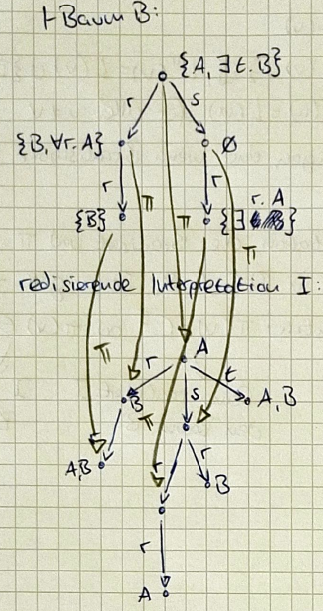
\includegraphics[width=2.0in,height=4.0in]{media/47real.png}

\begin{proposition}{Vollständigkeit}

Wenn $C_{0}$ erfüllbar, so gibt der Tableau-Algorithmus „erfüllbar``
zurück.
\end{proposition}

\textbf{T4.8}

\begin{proof}

Per Induktion über $\MI$. 

Sei $C_{0}$ erfüllbar. Nach \protect\hyperlink{proposition-4.5-terminierung}{Proposition 4.5} berechnet der Algorithmus endlich Folge $M_{0},\ldots,M_{n}$. Wir
zeigen: 

$M_{i}$ ist realisierbar für alle $0 \leq i \leq n$. 

Daraus folgt: Es gibt realisierbaren Baum $B \in M_{n}$ und damit enthält $B$ keinen offensichtlichen Widerspruch. Also gibt der Algorithmus „erfüllbar`` zurück.

\textbf{I.A.} $i = 0$. $M_{0} = {\{ B}_{\text{ini}}\}$.
$B_{\text{ini}}$ ist realisierbar, weil $C_{0}$ erfüllbar.

\textbf{I.S.} Fallunterscheidung gemäß der Regel, mit der $M_{i + 1}$
aus $M_{\MI}$ erzeugt wurde. Sei $B$ realisierbarer Baum aus
$M_i$, auf welchen Regel angewandt wird. Beispielhaft
$\sqcup$-Regel:

\begin{enumerate}
\def\labelenumi{\arabic{enumi}.}
\item
  $\sqcup$-Regel
\end{enumerate}

\begin{quote}
Dann wird $B = \left( V,E,L \right)$ ersetzt durch
$B^{'} = \left( V,E,L^{'} \right) \in M_{i + 1}$ und
$B^{''} = \left( V,E,L^{''} \right) \in M_{i + 1}$ und es gibt
$v \in V$ mit

\begin{itemize}
\item
  $\left( C \sqcup D \right) \in L(v)$
\item
  $L^{'}\left( v \right) = L\left( v \right) \cup \left\{ C \right\}$,
  $L^{''}\left( v \right) = L\left( v \right) \cup \left\{ D \right\}$
\item
  $L^{'}\left( u \right) = L^{''}\left( u \right) = L\left( u \right)$
  für alle $u \neq v$
\end{itemize}

Es genügt zu zeigen, dass wenn $B$ realisiertbar, dann $B'$ oder
$B''$ realisierbar. 

Sei $\MI$ Interpretation, die $B$ realisiert und $\pi\ :V \rightarrow \Delta^{\MI}$ Abbildung wie in \protect\hyperlink{realisierbarkeit}{Definition 4.8}. Dann gilt $\pi\left( v \right) \in \left( C \sqcup D \right)^{\MI}$. Nach Semantik: $\pi\left( v \right) \in C^{\MI}$ oder $\pi\left( v \right) \in D^{\MI}$. Also realisiert $\MI$ den Baum $B'$ oder $B''$.
\end{quote}
\end{proof}

\subsubsection{Komplexitätsanalyse}\label{praktikabilituxe4t}

Wir beobachten: 

I-Bäume können höchstens exponentiell groß werden.

Dieser Fall kann tastsächlich eintreffen. Beispielhaft, der Erfüllbarkeitstest von:
$$\bigsqcap_{i < n} \forall r^i .(\exists r.B \sqcap \exists r.\neg B)$$
generiert Baum der Größe $2^n$.

Also: exponentieller Zeit- und Platzverbrauch (sogar 2-exponentiell)

\subsubsection{Praktikabilität}

Offenbar wäre eine naive Implementierung nicht effizient. Dabei kann man aber einige Hinweise/Optimierungen bei der Implementierung beachten:

\begin{itemize}
	\item Es wird nur ein Baum zur Zeit generiert, keine Menge
	\item bei der $\sqcup$-Regel muss man sich also entscheiden (Heuristik); ggf. Entscheidung revidiieren (Backtracking).
	\item Es wird nur ein Teil des Baumes (Pfad) im Speicher gehalten.
	\item Backjumping: Führe Buch über die ``Herkunft'' von Knotenbeschriftungen und Kanten mittels Dependenzmengen. Wenn Backtracking nötig, springe direkt zu einer der Ursachen des Widerspruches zurück.
\end{itemize}

\subsection{ALC mit generellen TBoxen}\label{alc-mit-generellen-tboxen}

Nun wollen wir einen Tableau-Algorithmus für die Erfüllbarkeit in $\ALC$  \emph{bzgl. TBoxen}.

Jede TBox $\MT$ ist äquivalent zu einer TBox der Form
$\left\{ \top \sqsubseteq C_{\MT} \right\}$: 

\begin{center}setze $C_{\MT} := \prod_{C \sqsubseteq D \in \MT}^{}{\neg C \sqcup D}$.\end{center}

\textbf{T4.11} Beispiel

$$\MT = \{A \sqsubseteq \exists r.B, A \sqcup B \sqsubseteq \forall r.B\}$$

Daraus wird

$$\{\top \sqsubseteq (\neg A \sqcup \exists r.B) \sqcap (\neg (A \sqcup B) \sqcup \forall r.B)\}$$

in NNF:

$$\MT' = \{\top \sqsubseteq (\neg A \sqcup \exists r.B) \sqcap ((\neg A \sqcap \neg B) \sqcup \forall r.B)\}$$

Desweiteren nehmen wir an, dass:

\begin{itemize}
	\item Eingabe $C_0$ in NNF;
	\item Eingabe $\MT$ hat Form $\{\top \sqsubseteq C_{\MT}\}$ mit $C_{\MT}$ in NNF
\end{itemize}

Nun modifiziere den vorigen Algorithmus durch Hinzufügen folgender Regel:

\subsubsection{TBox-Regel}\label{tbox-regel}

Wähle $v \in V$ so dass $C_{\MT} \notin L\left( V \right)$ und
erweitere $L\left( v \right)$ um $C_{\MT}$.

Problem: Terminiert nicht!

\textbf{T4.12}

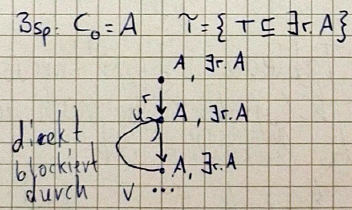
\includegraphics[width=3.71910in,height=1.83200in]{media/412endl.png}

\subsubsection{Blockieren}\label{blockieren}

Dies lösen wir, indem wir nur ein endliches Anfangsstück eines Baummodells anhand dessen sich die Existenzeines vollständigen Modells entscheiden lässt konstruieren. Dazu müssen wir die Anwendung der $\exists$-Regel einschränken.

\begin{definition}{Blockiert}

Sei $\left( V,E,L \right)$ ein I-Baum und $u,v \in V$. Dann ist
$v$ direkt blockiert durch $u$, wenn

\begin{enumerate}
\def\labelenumi{\arabic{enumi}.}
\item
  $u$ Vorgänger von $v$ in $B$ ist und
\item
  $L\left( v \right) \subseteq L\left( u \right)$
\end{enumerate}

$v$ ist blockiert, wenn $v$ direkt blockiert ist oder einen direkt
blockierten Vorgänger hat.
\end{definition}

\subsubsection{\texorpdfstring{Neue $\exists$-Regel
($\exists^{'}$-Regel)}{Neue \textbackslash{}exists-Regel (\textbackslash{}exists\^{}\{'\}-Regel)}}\label{neue-exists-regel-exists-regel}

\begin{itemize}
\item
  Wähle $v \in V$ und $\exists r.C \in L\left( v \right)$ so dass
  $v$ \emph{nicht blockiert ist und} es kein $v^{'} \in V$ gibt mit
  $\left( v,r,v^{'} \right) \in E$ und $C\  \in L\left( v' \right)$
\item
  erweitere V um neuen Konten $v^{'}$ und $E$ um
  $\left( v,r,v^{'} \right)$; setze
  $L\left( v^{'} \right) = \left\{ C \right\}$
\end{itemize}

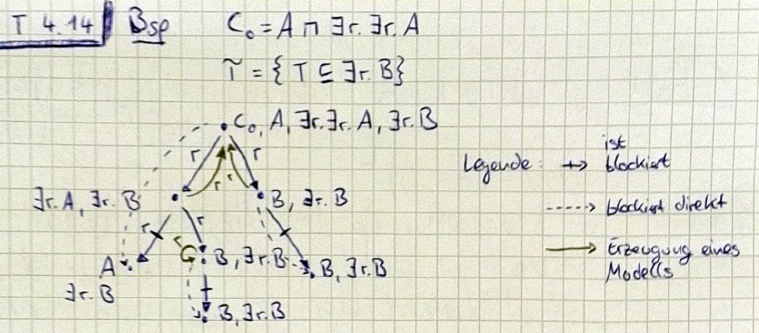
\includegraphics[width=5.71910in,height=2.33200in]{media/414block.png}

\subsubsection{Vollständigkeit}\label{vollstuxe4ndigkeit}

\begin{proposition}
Wenn $C_0$ erfüllbar bzgl. $\MT$, so gibt der Algorithmus erfüllbar zurück.
\end{proposition}

Beweis wie ohne TBoxen: Alle $M_{0},\ldots,\ M_{n}$ sind realisierbar
bzgl. $\MI$ (Induktion), also enthält $M_{n}$ einen Baum ohne
offensichtlichen Widerspruch (Nur neue Fallunterscheidung für TBox-Regel und Realisierbarkeitsbegriff auf TBoxen erweitert).

\subsubsection{Korrektheit}\label{korrektheit}

\begin{proposition}
Wenn der Algorithmus ``erfüllbar'' zurückgibt, so ist $C_0$ erfüllbar bzgl. $\MT$
\end{proposition}

\textbf{T4.15}

Beweisskizze per Induktion über die Struktur von $C$. Definiere
Interpretation $\MI$:

\begin{itemize}
\item
  $\Delta^{\MI} = \left\{ v \in V \middle| \text{v\ }\mathrm{\text{nicht\ blockiert}} \right\}$
\item
  $r^{\MI} = \left\{ \left( v,v^{'} \right)\  \middle| \ \left( v,r,v^{'} \right) \in E \right\} \cup \left\{ \left( v,u \right)\  \middle| \ \exists\left( v,r,v^{'} \right) \in E\mathrm{\ }\mathrm{\text{und}}\mathrm{\ }v^{'}\mathrm{\ }\mathrm{\text{direkt\ blockiert\ durch}}\mathrm{\ }u \right\}$
\item
  $A^{\MI} = \left\{ v \middle| A \in L\left( v \right) \right\}$
\end{itemize}

Behauptung: Für alle ALC-Konzepte $C$ und $v \in \Delta^{\MI}$ gilt:
$$C \in L\left( v \right) \Rightarrow v \in C^{\MI}$$
Die Behauptung impliziert wie gewünscht, dass

\begin{itemize}
\item
  $\MI$ Modell von $\MT$ ist.

Da die TBox-Regel nicht anwendbar ist, gilt $C_{\MT} \in L\left( v \right)$ für alle $v \in V$. Also $v \in C_{\MT}^{\MI}$ für alle $v \in \Delta^{\MI}$.

\item
  $\MI$ Modell von $C_{0}$ ist.

Da $C_{0} \in L\left( v_{\text{ini}} \right)$ gilt nach Behauptung
$v_{\text{ini}} \in C_{0}^{\MI}$.
\end{itemize}

\textbf{I.A.} Siehe Beweis zu
\protect\hyperlink{proposition-4.7-korrektheit}{Proposition 4.7}.

\textbf{I.S.} Schritte wie in Beweis zu Proposition 4.7, außer:

\begin{itemize}
\item
  $C = \exists r.D$
\end{itemize}

Sei $\exists r.D \in L\left( v \right)$. Da die $\exists'$-Regel
nicht anwendbar ist, gibt es $v^{'} \in V$ mit
$\left( v,r,v^{'} \right) \in E$ und $D \in L\left( v \right)$.
Fallunterscheidung:

\begin{enumerate}
\def\labelenumi{\arabic{enumi}.}
\item
  $v'$ unblockiert. Dann $\left( v,v^{'} \right) \in r^{\MI}$
  (Definition $\MI$), $v^{'} \in D^{\MI}$ (\textbf{I.V.})
  $\Rightarrow v \in \left( \exists r.D \right)^{\MI}$
\item
  $v^{'}$ blockiert. Da der direkte Vorgänger $v$ von $v'$
  unblockiert ist, ist $v'$ direkt blockiert von unblockiertem
  Vorgänger $u$. Es gilt:
\end{enumerate}

\begin{itemize}
\item
  $\left( v,u \right) \in r^{\MI}$ nach Definition $r^{\MI}$
\item
  $D \in L\left( v \right) \subseteq L\left( u \right)$
  (Blockierungsbedingung)
\item
  $\Rightarrow u \in D^{\MI}$ (\textbf{I.V.})
\end{itemize}

\begin{quote}
Also $v \in \left( \exists r.D \right)^{\MI}$.
\end{quote}

\begin{itemize}
\item
  $C = \forall r.D$
\end{itemize}

Ähnlich zu oberem Fall.

\subsubsection{Terminierung}\label{terminierung}

\begin{proposition}
Der Tableau-Algorithmus stoppt nach endlicher Zeit.
\end{proposition}

Beweis analog zu den ohne TBoxen (Prop. 4.5), aber mit Einbezug der TBox. Wir zeigen es also in den selben Schritten:

Beweis in 4 Schritten:

\begin{enumerate}
\def\labelenumi{\arabic{enumi}.}
\item
  Es werden nur I-Bäume mit einem Verzweigungsgrad $\leq \left| C_{0} \right| + \color{red} \left| \MT \right|$ generiert.
\item
  Es werden nur I-Bäume mit einer Tiefe $\color{red} 2^k$ generiert.
  \begin{quote}
  \textbf{T4.16}

  Angenommen, es wird ein I-Baum der Tiefe $> 2^k$ erzeugt.

  Dann wird irgendwann die $\exists '$-Regel auf einen Knoten $v$ der Tiefe $2^k$ angewendet.

  Betrachte Pfad $v_0, \ldots , v_{2^k}$ von der Wurzel bis v. Dieser Pfad hat $2^k+1$ Knoten.

  Weil es nur $2^k$ möglich Knotenbeschriftungen gibt, muss es auf dem Pfad zwei Knoten $v_i$ und $v_j$ geben, mit $0 \leq i < j \leq 2^k$, welche dieselben Knotenbeschriftungen haben, also $L(v_i) = L(v_j)$. Also ist $v_j$ durch $v_i$ blockiert, weswegen auch $v$ blockiert ist. $\lightning$

  Widerspruch zur Anwendung der $\exists '$-Regel auf $v_j$, also ist die Annahme falsch.
  \end{quote}
\item
  Sei $M_{0},M_{1},\ldots$ die erzeugte Folge und $B \in M_{\MI}$ für
  ein $i \geq 0$. Dann ist $B$ durch die Anwendung von maximal
  $\color{red} k^{2^{k}} \cdot k \leq 2^{2^{3k}}= n$ Regeln entstanden (Knoten im Baum mal Größe Knotenbeschriftung).
\end{enumerate}

Danach kann Terminierung wie gehabt mittels Behauptung 3 bewiesen werden.

\subsubsection{Komplexität}

Im Beweis zum 3. Schritt der Terminierung haben wir gesehen, dass die I-Bäume höchstens doppelt exponentiell groß werden.

Dieser Worst-Case kann eintreten!

\begin{lemma}
Es gibt Eingabe $C_0$, $\MT$ für die der Tableau-Algorithmus einen Baum von exponentieller Tiefe generiert.
\end{lemma}

Also: 2-exponentieller Zeit- und Platzaufwand (sogar 3-exponentiell!).

\subsubsection{Bemerkung zur TBox-Regel}

\subsubsection{Erweiterungen}